\documentclass[12pt,a4paper,twoside]{report}
	\makeatletter
	\def\@makechapterhead#1{%
  	%%%%\vspace*{50\p@}% %%% removed!
  	{\parindent \z@ \raggedright \normalfont
    	\ifnum \c@secnumdepth >\m@ne
        	\huge\bfseries \@chapapp\space \thechapter
        	\par\nobreak
        	\vskip 20\p@
    	\fi
    	\interlinepenalty\@M
    	\Huge \bfseries #1\par\nobreak
    	\vskip 40\p@
  	}}
	\def\@makeschapterhead#1{%
  	%%%%%\vspace*{50\p@}% %%% removed!
  	{\parindent \z@ \raggedright
    	\normalfont
    	\interlinepenalty\@M
    	\Huge \bfseries  #1\par\nobreak
    	\vskip 40\p@
  	}}
	\makeatother

\usepackage[utf8]{inputenc}
\usepackage[german]{babel}
\usepackage[T1]{fontenc}
\usepackage{amsmath}
\usepackage{amsfonts}
\usepackage{amssymb}
\usepackage{makeidx}
\usepackage{graphicx}
    \graphicspath{ {./images/} }
\usepackage[hidelinks]{hyperref}
	\hypersetup{
		colorlinks,
		allcolors=black
	}
\usepackage{caption}
\usepackage{subcaption}
\usepackage{pdfpages}
\usepackage{wrapfig}
\usepackage{kpfonts}
\usepackage[a4paper, width=150mm, top=25mm, bottom=25mm, bindingoffset=6mm]{geometry}
\usepackage{fancybox}
\usepackage{fancyvrb}
\usepackage{fancyhdr}
    \pagestyle{fancy}
    \fancyhead{}
    \fancyhead[RO,LE]{Kapitel \thechapter}
\usepackage{array}
\usepackage{tabularx}
\usepackage{booktabs}
\usepackage{longtable}
\usepackage{acronym}
\usepackage{csquotes}
\usepackage[backend=biber, bibencoding=utf8, style=ieee, dashed=false]{biblatex}
\addbibresource{bibliography/bib.bib}

\title{Entwicklung eines Prüfgeräts für Druckschalter}
\author{Jan Möllering}
\date{15.09.2021}


\begin{document}
\emergencystretch 3em

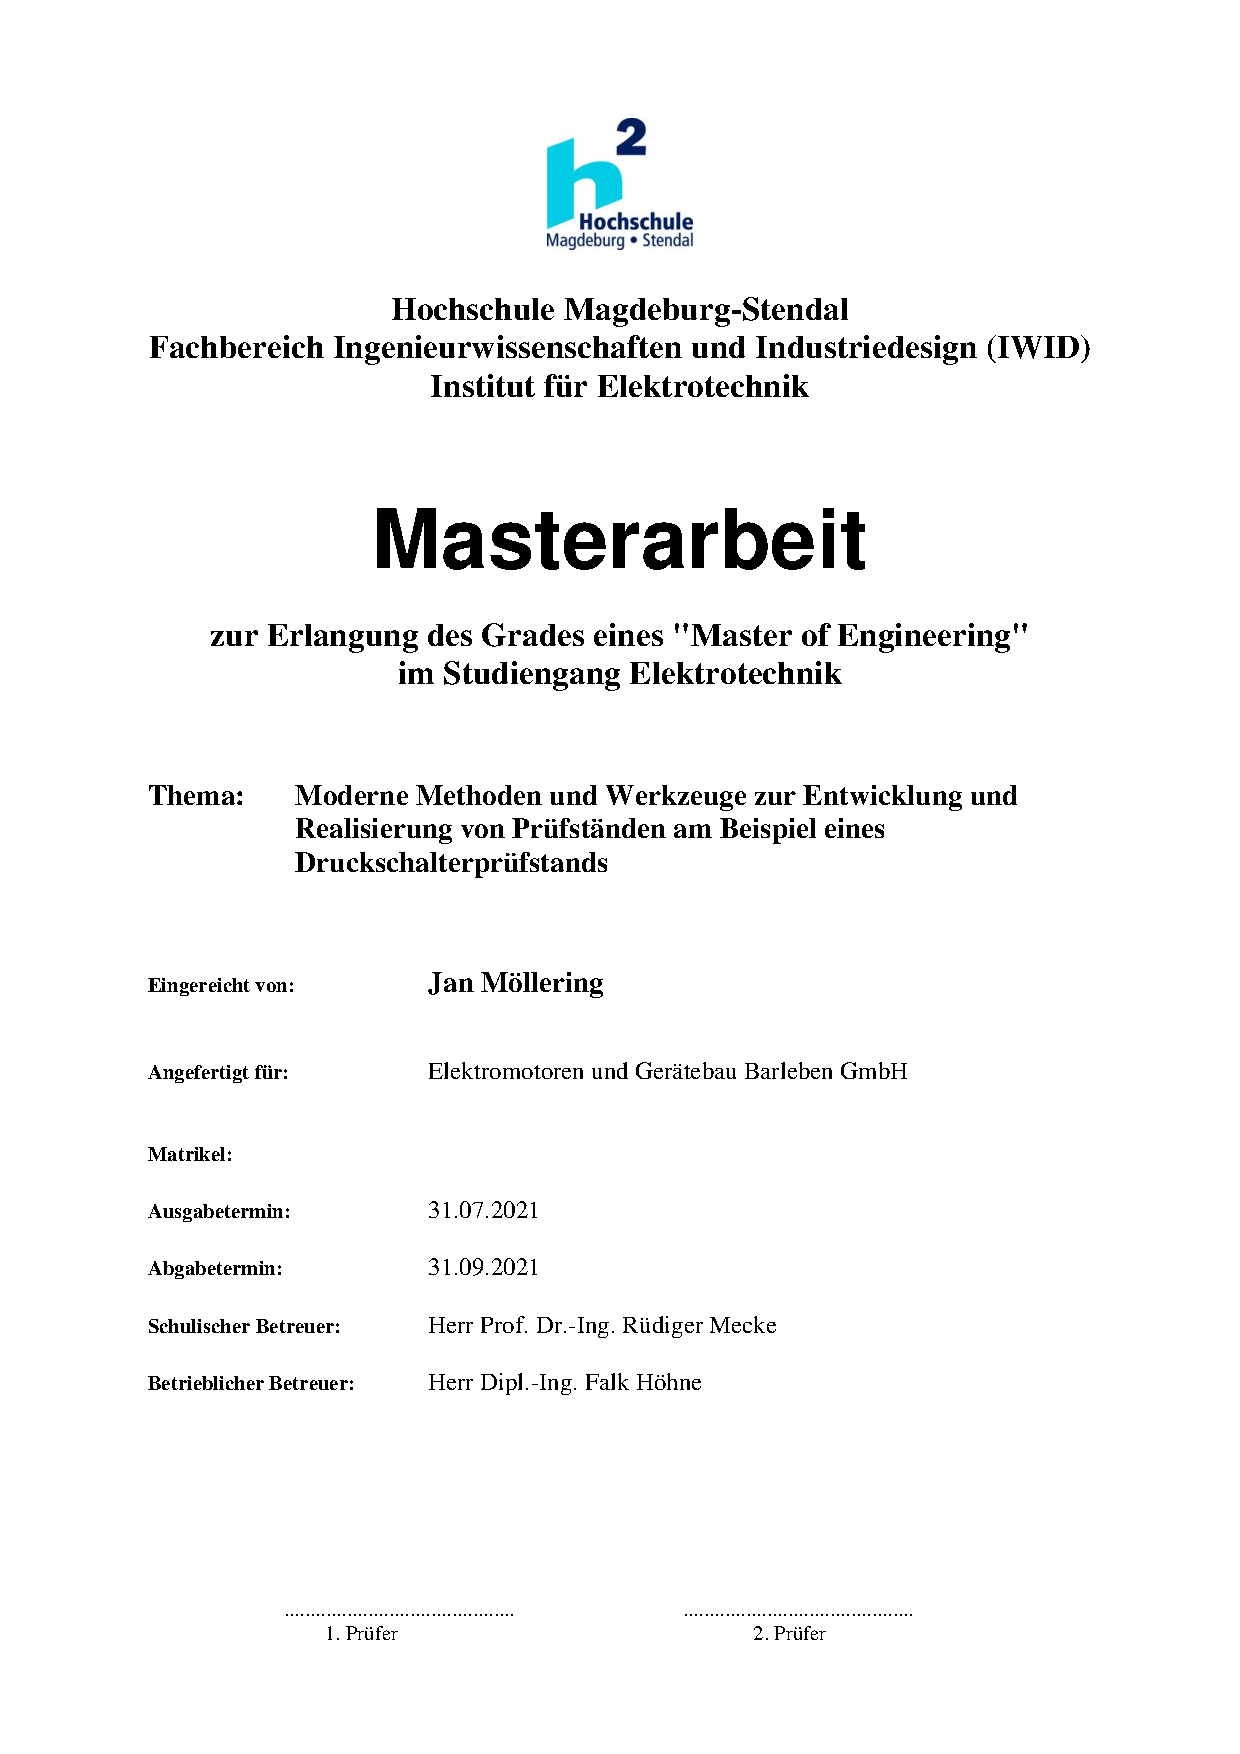
\includepdf{Musterdeckblatt_Master.pdf}

\chapter*{Eidesstattliche Erklärung}
\thispagestyle{empty}
Hiermit erkläre ich, dass ich die vorliegende Arbeit eigenständig
und ohne fremde Hilfe angefertigt habe.
Textpassagen, die wörtlich oder dem Sinn nach auf Publikationen
oder Vorträgen anderer Autoren beruhen, sind als solche kenntlich gemacht.
\\
\noindent
Die Arbeit wurde bisher keiner anderen Prüfungsbehörde vorgelegt
und auch noch nicht veröffentlicht.

\vspace{4cm}

\hspace{1cm} Ort, Datum \hfill Unterschrift \hspace{2cm}

\chapter*{Abstract}
\thispagestyle{empty}
Diese Arbeit beschäftigt sich mit der Entwicklung eines Prüfgeräts für Druckschalter.
\\
\\
\\
\\
\\
This Thesis is about the development of a measurement device for pressure switches.

\setcounter{tocdepth}{2}
\tableofcontents
\thispagestyle{empty}
\newpage
\pagenumbering{Roman}
\addtocontents{toc}{\protect\thispagestyle{empty}}


\addcontentsline{toc}{chapter}{Tabellenverzeichnis}
\listoftables
\newpage

\addcontentsline{toc}{chapter}{Abbildungsverzeichnis}
\listoffigures

\addcontentsline{toc}{chapter}{Abkürzungsverzeichnis}
\chapter*{Abkürzungsverzeichnis}
\begin{acronym}[slmtA]
	\acro{GmbH}{Gemeinschaft mit beschränkter Haftung}
	\acro{USD}{United States Dollar}
	\acro{CSV}{Comma Seperated Values}
	\acro{PDF}{Portable Document Format}
	\acro{USB}{Universal Serial Bus}
	\acro{I2C}{Inter-Intergrated Circuit}
	\acro{UART}{Universal Asynchronous Receiver/Transmitter}
	\acro{HDMI}{High-Definition Multimedia Interface}
	\acro{IPC}{Inter Process Communication}
	\acro{DOM}{Document Object Model}
	\acro{LED}{Light Emmitting Diode}
	\acro{ADC}{Analog-to-Digital Converter}
	\acro{RTOS}{Real Time Operating System}
	\acro{OS}{Operating System}
	\acro{API}{Application Programming Interface}
	\acro{HTML}{Hypertext Markup Language}
	\acro{CSS}{Cascading Style Sheets}
	\acro{SCL}{System Clock}
	\acro{SDA}{System Data}
	\acro{JSON}{JavaScript Object Notation}
	\acro{XML}{Extensible Markup Language}
	\acro{SAR}{Successive Approximation Register}
	\acro{DAC}{Digital-to-Analog Converter}
	\acro{Mio}{Millionen}
	\acro{FiFo}{First in First out}
\end{acronym}
\newpage

\chapter{Motivation und Aufgabenstellung}
\pagenumbering{arabic}
\setcounter{page}{1}
\section{Motivation}
\clearpage

\section{Aufgabenstellung}

\textbf{Die Teilaufgaben umfassen:}

\begin{itemize}
	\item Einarbeitung in die ...
	\item Entwicklung der Elektronik für das Prüfgerät
	\begin{itemize}
		\item Unterpunkt 1
		\item Unterpunkt 2
		\item Messen von Stromwerten im \(\mu\)A Bereich
	\end{itemize}
	\item Entwicklung und Programmierung der Software für das Prüfgerät
	\begin{itemize}
		\item Steuerung des Prüfgeräts
		\item Darstellung, Speicherung und Auswertung der Messwerte
		\item Realisierung einer grafischen Oberfläche
	\end{itemize}
	\item Auswahl aller benötigten Komponenten
	\item Aufbau eines funktionsfähigen Prototyps des Prüfgeräts
	\item Erprobung und Testung von Teilkomponenten
\end{itemize}
\clearpage

\section{Detaillierte Anforderungen an das Prüfgeräts}
Im Folgenden ist eine detailliertere Beschreibung der Anforderungen an den Prüfstand aufgelistet.
Diese Anforderungen haben sich in Absprache mit der Abteilung Technik ergeben.

\chapter{Funktionsweise CF38, Druckschalter, HTS-Levelschalter}
\section{Funktionsweise CF38}

\section{Funktionsweise Druckschalter}

\section{Funktionsweise HTS-Levelschalter}

\chapter{Entwicklung des Prüfgeräts}
\section{Anforderungen und Funktionen}

\section{Marktanalyse / Recherche}

\section{Entwicklung der Strommessung}

\section{Entwicklung des HMI}

\section{Entwicklung der integrierten Spannungsversorgung}

\section{Entwicklung der Steuerung}

\section{Entwicklung der Platine}

\chapter{Erprobung und Ergebnisse}
\section{Genauigkeit}

\section{Stabilität}

\section{Präzision}

\section{Bewertung durch ein Prüflabor}

\section{Diskussion der Ergebnisse}

\chapter{Zusammenfassung und Ausblick}

\printbibliography

\appendix

\chapter{Datenblätter}
\newpage

\chapter{Schalt- und Stromlaufpläne}

\end{document}